    %package list
    \documentclass{article}
    \usepackage[english,spanish]{babel}
    \usepackage[utf8]{inputenc}
    \usepackage[top=3cm, bottom=3cm, outer=3cm, inner=3cm]{geometry}
    \usepackage{multicol}
    \usepackage{graphicx}
    \usepackage{url}
    \usepackage{hyperref}
    \usepackage{array}
    \newcolumntype{x}[1]{>{\centering\arraybackslash\hspace{0pt}}p{#1}}
    \usepackage{natbib}
    \usepackage{pdfpages}
    \usepackage{multirow}
    \usepackage[normalem]{ulem}
    \useunder{\uline}{\ul}{}
    \usepackage{svg}
    \usepackage{xcolor}
    \usepackage{listings}
    \usepackage{caption}
    \usepackage{subcaption}
    \usepackage{float}
    \usepackage{array}
    \usepackage[english,spanish]{babel}
    \usepackage[utf8]{inputenc}
    \usepackage{fancyhdr}
    \usepackage{listings}
    \usepackage{color, colortbl}
    \usepackage{amsmath}

    \lstdefinestyle{ascii-tree}{
        literate={├}{|}1 {─}{--}1 {└}{+}1 
    }
    
    \lstset{basicstyle=\ttfamily,
    showstringspaces=false,
    commentstyle=\color{red},
    keywordstyle=\color{blue}
    }

    \newcolumntype{M}[1]{>{\centering\arraybackslash}m{#1}}
    \newcolumntype{N}{@{}m{0pt}@{}}

    %%%%%%%%%%%%%%%%%%%%%%%%  ITEMS  %%%%%%%%%%%%%%%%%%%%%%%%%%%%%%%%%

    \newcommand{\itemUniversity}{Universidad Nacional de San Agustín de Arequipa}
    \newcommand{\itemFaculty}{Facultad de Ingeniería de Producción y Servicios}
    \newcommand{\itemSchool}{Escuela Profesional de Ingeniería de Sistemas}
    \newcommand{\itemCourse}{Estructura de datos y Algoritmos}
    \newcommand{\itemTheme}{Grafos}

    %%%%%%%%%%%%%%%%%%%%%%%%   HEADER   %%%%%%%%%%%%%%%%%%%%%%%%%%%%%%

    \AtBeginDocument{\selectlanguage{spanish}}
    \renewcommand{\figurename}{Figura}
    \renewcommand{\refname}{Referencias}
    \renewcommand{\tablename}{Tabla} 
    \AtBeginDocument{%
        \renewcommand\tablename{Tabla}
    }

    \pagestyle{fancy}
    \fancyhf{}
    \setlength{\headheight}{30pt}
    \renewcommand{\headrulewidth}{1pt}
    \renewcommand{\footrulewidth}{1pt}

    \fancyhead[L]{\raisebox{-0.2\height}{
\includegraphics[width=3cm]{img/logo_episunsa.png}}}
    \fancyhead[C]{\fontsize{7}{7}\selectfont	\itemUniversity \\ \itemFaculty \\ \itemDepartment \\ \itemSchool \\ \textbf{\itemCourse}}
    \fancyhead[R]{\raisebox{-0.2\height}{
\includegraphics[width=1.2cm]{img/logo_abet}}}

    \fancyfoot[L]{Reyser Z. - Jhastyn P.}
    \fancyfoot[C]{\itemCourse}
    \fancyfoot[R]{Página \thepage}

    % para el codigo fuente
    \definecolor{dkgreen}{rgb}{0,0.6,0}
    \definecolor{gray}{rgb}{0.5,0.5,0.5}
    \definecolor{mauve}{rgb}{0.58,0,0.82}
    \definecolor{codebackground}{rgb}{89, 0.97, 0.90}
    \definecolor{tablebackground}{rgb}{0.8, 0, 0}

    \lstset{frame=tb,
        language=bash,
        aboveskip=3mm,
        belowskip=3mm,
        showstringspaces=false,
        columns=flexible,
        basicstyle={\small\ttfamily},
        numbers=none,
        numberstyle=\tiny\color{gray},
        keywordstyle=\color{blue},
        commentstyle=\color{dkgreen},
        stringstyle=\color{mauve},
        breaklines=true,
        breakatwhitespace=true,
        tabsize=3,
        backgroundcolor= \color{codebackground},
    }

    %%%%%%%%%%%%%%%%%%%%%%   CARATULA  %%%%%%%%%%%%%%%%%%%%%%%%%%%%%%%%%
    \begin{document} 
        \begin{titlepage}
        \centering
        
        {\bfseries\LARGE {\itemUniversity} \par} \vspace{0.3 cm}
        {\scshape\Large {\itemFaculty} \par} \vspace{0.3 cm}
        {\scshape\Large {\itemSchool} \par}\vspace{1 cm}

        {
\includegraphics[width=0.4\textwidth]{{img/logo_unsa_corto.png}}\par}
        \vspace{0.5 cm}
        
        {\scshape\LARGE  INFORME DE LABORATORIO 08 \par}
        {\scshape\Large {\itemCourse} \par}
        \vspace{1 cm}
        
        {\Large Alumnos:\par}
        {\begin{itemize} \centering 
            \item {\Large Payehuanca Riquelme Jhastyn Jefferson\par}
            \item {\Large Zapata Butron Reyser Julio\par}
        \end{itemize}}
        \vspace{0.5 cm}
        
        {\Large Docente:\par}
        {\Large Quispe Vergaray Karen Melissa\par}
        \vfill
        \vspace{1 cm}
        
        {\Large 28 de diciembre 2023 \par}
        {\Large Arequipa - Perú \par}
        
        \end{titlepage}
    %%%%%%%%%%%%%%%%%%%%%%   CONTENIDO   %%%%%%%%%%%%%%%%%%%%%%%%%%%%%%%%%
    
        \vspace*{2px}
        
        \begin{center}	
            \fontsize{17}{17} \textbf{Informe Laboratorio 08}
        \end{center}
    
        \centerline{\textbf{\Large Tema: \itemTheme}}

    %%%%%%%   REPOSITORIO   %%%%%%% 
        \section{URL de Repositorio Github}
            \textbf{Link del Repositorio en Github: }    
                \url{https://github.com/ReyserLyn/Eda_lab08.git}

    %%%%%%%   EJERCICIOS   %%%%%%%     
        
        \section{Ejercicios designados}

        \begin{enumerate}
            \item Crear un repositorio en GitHub, donde incluyan la resolucion de los ejercicios propuestos y el informe. 
            \item Implementar el cogido de Grafo cuya representacion sea realizada mediante LISTA DE ADYACENCIA. (3 puntos) 
            \item Implementar BSF, DFS y Dijkstra con sus respectivos casos de prueba. (5 puntos)
            \item Solucionar el siguiente ejercicio: (5 puntos) \\
            El grafo de palabras se define de la siguiente manera: cada vértice es una palabra en el idioma Inglés y dos palabras son adyacentes si difieren exactamente en una posición. Por ejemplo, las cords y los corps son adyacentes, mientras que los corps y crops no lo son. 
            
            {\begin{itemize}
                \item Dibuje el grafo definido por las siguientes palabras: words cords corps coops crops drops drips grips gripe grape graph.
                \item Mostrar la lista de adyacencia del grafo.
            \end{itemize}}

            \item Realizar un metodo en la clase Grafo. Este metodo permitira saber si un grafo esta incluido en otro. Los parametros de entrada son 2 grafos y la salida del metodo es true si hay inclusion y false el caso contrario. (4 puntos)
        \end{enumerate} 

    %%%%%%%   SOLUCIÓN   %%%%%%%     
        \section{Solución}
        
            \subsection{Clase GraphLink}\par  

                Este es la clase más importante y más compleja del trabajo, puesto que responde correctamente a los ejercicios designados.
                
                \lstinputlisting[language=Java, caption={GraphLink.java},numbers=left,]{src/GraphLink.java}

                \begin{itemize}
                    \item \texttt{insertVertex(E data): String}\\
                    Inserta un nuevo vértice con el dato \texttt{data} en el grafo. Retorna un mensaje indicando si la operación fue exitosa.
                    
                    \item \texttt{insertEdge(E dataOri, E dataDes): void}\\
                    Inserta una arista entre los vértices con datos \texttt{dataOri} y \texttt{dataDes}. Lanza una excepción si alguno de los vértices no existe.
                    
                    \item \texttt{insertEdge(E dataOri, int weight, E dataDes): void}\\
                    Inserta una arista ponderada entre los vértices con datos \texttt{dataOri} y \texttt{dataDes} con el peso especificado. Lanza una excepción si alguno de los vértices no existe.
                    
                    \item \texttt{removeEdge(E dataOri, E dataDes): void}\\
                    Elimina la arista entre los vértices con datos \texttt{dataOri} y \texttt{dataDes}. Lanza una excepción si alguno de los vértices no existe.
                    
                    \item \texttt{removeEdge(E dataOri, int weight, E dataDes): void}\\
                    Elimina la arista ponderada entre los vértices con datos \texttt{dataOri} y \texttt{dataDes} con el peso especificado. Lanza una excepción si alguno de los vértices no existe.
                    
                    \item \texttt{removeVertex(E x): String}\\
                    Elimina el vértice con el dato \texttt{x} y todas las aristas asociadas. Retorna un mensaje indicando si la operación fue exitosa.
                    
                    \item \texttt{searchEdge(E dataOri, E dataDes): boolean}\\
                    Verifica si existe una arista entre los vértices con datos \texttt{dataOri} y \texttt{dataDes}. Lanza una excepción si alguno de los vértices no existe.
                    
                    \item \texttt{searchEdge(E dataOri, int weight, E dataDes): boolean}\\
                    Verifica si existe una arista ponderada entre los vértices con datos \texttt{dataOri} y \texttt{dataDes} con el peso especificado. Lanza una excepción si alguno de los vértices no existe.
                    
                    \item \texttt{searchVertex(E data): boolean}\\
                    Verifica si existe un vértice con el dato \texttt{data} en el grafo.
                    
                    {\item \texttt{buscarElemento(E data): Vertex<E>}\\
                    Busca y retorna el vértice con el dato \texttt{data} en el grafo.}
                    
                    {\item \texttt{getListVertex(): ListLinked<Vertex<E\>\>}\\
                    Retorna la lista de vértices del grafo.}
                    
                    \item \texttt{bfs(E startData): void}\\
                    Realiza un recorrido en amplitud (BFS) desde el vértice con dato \texttt{startData} e imprime los vértices visitados.
                    
                    \item \texttt{dfs(E startData): void}\\
                    Realiza un recorrido en profundidad (DFS) desde el vértice con dato \texttt{startData} e imprime los vértices visitados.
                    
                    \item \texttt{dijkstra(E startData, E endData): int}\\
                    Calcula la distancia mínima entre los vértices con datos \texttt{startData} y \texttt{endData} utilizando el algoritmo de Dijkstra.
                    
                    \item \texttt{isIncludedIn(GraphLink<E> otherGraph): boolean}\\
                    Verifica si el grafo actual está incluido en otro grafo (\texttt{otherGraph}).
                    
                    \item \texttt{toString(): String}\\
                    Retorna una representación en cadena del grafo.
                \end{itemize}

            \subsection{Clase Main}

                Este es la clase en el que se hace un test de las clases realizadas y se encarga de responder los ejercicios designados, cumpliendo con lo que se pide y mostrando todo lo necesario.
            
                \lstinputlisting[language=Java, caption={Main.java},numbers=left,]{src/Main.java}

                Ejecutando nuestro Main, se evidencia el cumplimiento de los ejercicios designados. A continuación capturas de la ejecución.

            \subsection{Ejecución}
                \begin{center}
                    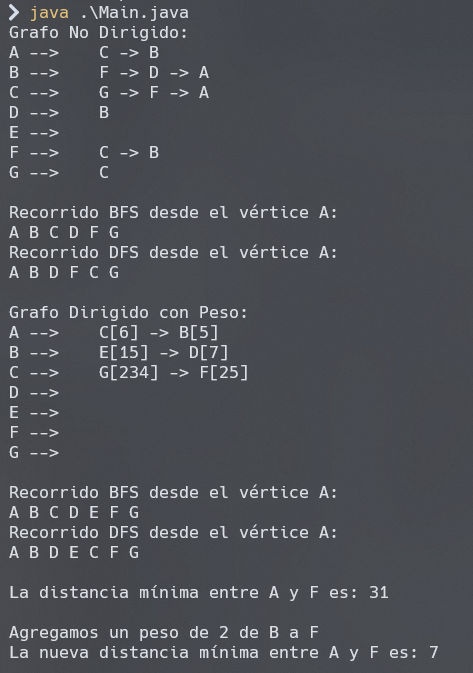
\includegraphics[width=0.55\textwidth]{img/cap1.png}
                \end{center}

                \begin{center}
                    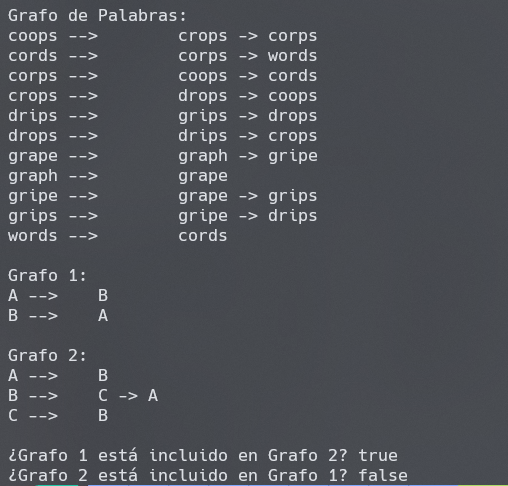
\includegraphics[width=0.55\textwidth]{img/cap2.png}
                \end{center}

    %%%%%%%   CUESTIONARIO   %%%%%%%     
                
        \section{Cuestionario}    

        \begin{enumerate}
            \item {\textbf{¿Cuantas variantes del algoritmo de Dijkstra hay y cuál es la diferencia entre ellas? (1 puntos)}} \\
            Hay dos variantes principales del algoritmo de Dijkstra: el algoritmo original y la versión con cola de prioridad. La principal diferencia radica en la implementación de la estructura de datos para manejar los vértices no visitados. La versión con cola de prioridad es más eficiente en términos de tiempo de ejecución, ya que mejora la complejidad temporal del algoritmo.

            \item {\textbf{Invetigue sobre los ALGORITMOS DE CAMINOS MINIMOS e indique, ¿Qué similitudes encuentra, qué diferencias, en qué casos utilizar y porque? (2 puntos)}}\\
            Los algoritmos de caminos mínimos, como Dijkstra y Bellman-Ford, comparten la meta de encontrar la ruta más corta entre dos puntos en un grafo ponderado. La principal diferencia es que Dijkstra se utiliza para grafos con pesos no negativos, mientras que Bellman-Ford puede manejar pesos negativos, aunque con una complejidad temporal mayor.
        \end{enumerate}

    %%%%%%%   CONCLUSIONES   %%%%%%%     

        \section{Conclusiones}
            \begin{itemize}
                \item La representación de grafos mediante listas de adyacencia ofrece flexibilidad y eficiencia para diversas operaciones, facilitando la implementación de algoritmos como DFS, BFS, y Dijkstra.
                \item La modularidad y reutilización de código se favorecen mediante la implementación de clases y métodos específicos, permitiendo construir y mantener sistemas más complejos con facilidad.
                \item Trabajar con clases propias en lugar de importar bibliotecas externas ofrece mayor control y comprensión sobre el funcionamiento interno del código. 
            \end{itemize}
            
    %%%%%%%   REFERENCIAS   %%%%%%% 
        \section{Referencias}
        
        \begin{itemize}			
            \item \url{https://www.ecured.cu/Algoritmo_de_Dijkstra}
            \item \url{https://www.geeksforgeeks.org/difference-between-bfs-and-dfs/}
            \item \url{https://runestone.academy/ns/books/published/pythoned/Graphs/UnaListaDeAdyacencia.html}     
        \end{itemize}	

    %%%%%%%   END   %%%%%%% 
    \end{document}